
\clearpage

\section{Una revisión al ADN}
\label{sec:ADN}


\subsection{Historia del ADN}
La epopeya del ADN tiene sus inicios en 1869 con un bioquímico llamado Friedrich Miescher, esté estaba interesado en la estructura química de las fascinantes unidades fundamentales de la vida conocidas como células.
Miescher viajaba todos los días a la clínica más cercana para tomar las vendas sucias, esto debido a que estaban recubiertas de pus (lo cual era una buena fuente de leucocitos), añadiendo álcali hizo que los núcleos se abrieran liberando sus componentes, de esta manera Miescher extrajo un componente(ADN), al que el nombro nucleína, realizando un análisis de esta nucleína mostró que era un ácido que contenía fósforo y por tanto no calificaba en en ninguno de los grupos conocidos en ese momento como carbohidratos y proteínas, este fue clasificado como un ácido nucleico y su relevancia biológica no fue descubierta hasta mucho tiempo después \cite{Susan}.\\

En 1928 Fredrick Griffith realizaba una investigación con neumococos, tenia dos tipos: el primero patógeno  fue cultivado en placas de petri conocido como s(smooth-suave) debido a su apariencia, el segundo inofensivo y conocido como r(rough-áspero), Griffith descubrio que al añadir un extracto de los neumococos tipos S al tipo R, esté ultimo podría heredar las propiedades del tipo S, este -principio de transformación- indicaba que el extracto contenía la molécula de herencia.\\

Oswald Avery junto con MacLeod y McCarty demostrarón que substancia efectiva en el experimento de Griffiths era la molecula de ADN y que a su vez, era el portador de genes en la célula, también es importante mencionar que Alfred Hershey y Martha Chase quienes confirmaron la conclusión en 1952 mediante experimentos con trazadores radioactivos\cite{Thormod}.\\

Es relevante mencionar otros aportes significativos: \\
1.Erwin Chargaff encontro una regularidad peculiar en los radios de las bases de los nucleotidos.\\
2.Sven Furger trabajo en la estructura de los componentes del ADN, encontró que la base plana(plano de la citocina) era perpendicular a la molecula de azucar.\\
3.Rosalind Franklin logro distinguir dos tipos de ADN dependiendo de la hidratación y que ambos tenían estructura helicoidal mediante cristalográfia, véase figura ~\ref{fig:rf}.

\begin{figure}[htbp]
    \centering
    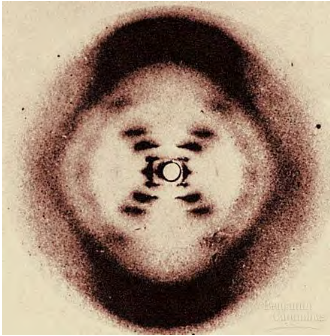
\includegraphics[width=0.5\linewidth]{./Figures/RF.png}
    \caption[Fotografía cristalográfica del ADN]{Fotografiá cristalográfica del ADN tomada por Rosalind Franklin en 1952}
    \label{fig:rf}
\end{figure}
El ultimo paso hacia la estructura del ADN fue llevado acabo por James Watson y Francis Crick en el laboratorio de Cavendish en francia, juntos trabajaron en diferentes modelos de la molécula de ADN , en 1953 publicaron un articulo en la prestigiosa revista Nature titulado: "Molecular Structure of Nucleid Acids", el articulo solo tenia una pagina, pero era de un impacto significativo debido al modelo de ADN que contenía, un modelo de doble hélice(figura ~\ref{fig:jw}), y sugerían que el emparejamiento  especifico que habían postulado intuía un posible mecanismo para copiar material genético.
\begin{figure}[htbp]
    \centering
    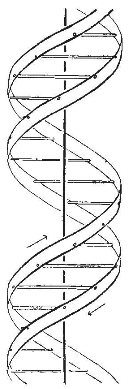
\includegraphics[width=0.15\linewidth]{./Figures/DNA1.png}
    \caption[Diagrama esquemático del ADN]{Diagrama esquemático del ADN publicado por Watson y Crick en 1953, imagen tomada de \cite{jwfc}.}
    \label{fig:jw}
\end{figure}
\subsection{Estructura del ADN}
Como ya se vio el ADN es una molécula compuesta por dos largas cadenas, estas cadenas estan formadas de múltiples nucleotidos y cada nucleotido esta compuesto por una base una molecula azúcar y un grupo fosfato, la base puede tener cuatro formas: citocina, timina, guanina y adenina. Una cadena de ADN se une a otra por medio de los enlaces de hidrógeno que se extienden entre pares base, entonces C se une específicamente con G, y A se une con T, de esta manera se forman los pares base C-G y A-T.
Es interesante mencionar que si todo el ADN de solo una célula humana fuera unido y estirado, tendría una longitud aproximada de dos metros de largo.


\subsubsection{Daño inducido por radiación al ADN}
En general existen cuatro tipos de daño en el ADN, estos pueden ser causados por exposición a luz uv, radiación ionizante, exposición química, errores de repiclación o metabolismo celular.
\paragraph{Rompimientos simples}
Un rompimiento simple es un rompimiento en un enlace peptidico, es decir azúcar fosfato, este daño es usualmente fácil de reparar, y en experimentos  se ha demostrado que aproximadamente el 90\% de los rompimientos simples son reparados en el curso de una hora a una temperatura de $37^{\circ} C$ \cite{Thormod}

\paragraph{Rompimientos dobles}

Este tipo de daño involucra las dos cadenas  del ADN, Si el enlace peptidico se rompe a cada lado dentro de una distancia de unos cuantos pares base se presentara un rompimiento doble, estos suelen estar relacionados con muerte celular y daño a los cromosomas.\\
Los rompimientos dobles son posibles de reparar, sin embargo, es mucho más difícil de reparar que un rompimiento simple,
la molécula de ADN contiene proteínas que suportan la estructura y previene que las piezas se caigan incluso cuando un rompimiento ocurre en ambas cadenas del ADN, de hecho, existen un numero de mecanismos que organismos complejos(como los humanos) han evolucionado para reparar los rompimientos dobles\cite{Thormod}.

\begin{figure}[htbp]
    \centering
    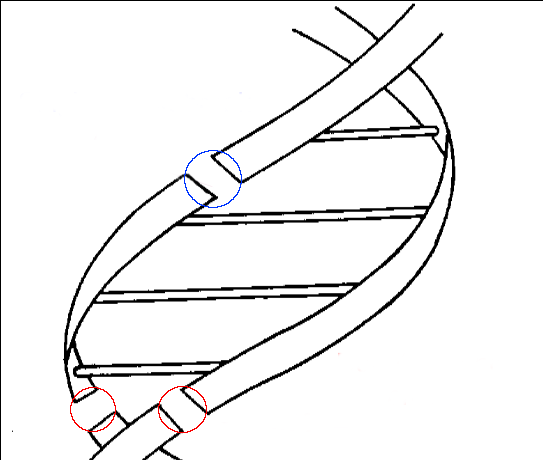
\includegraphics[width=0.5\linewidth]{./Figures/esbdb.png}
    \caption[Esquema rompimientos simples y dobles]{}
    \label{fig:esbdb}
\end{figure}


\paragraph{Daño base}

Como resultado de un fallo al reparar o de una falta de reparación, el codon(una secuencia de tres nucleótidos) alterado puede insertar un aminoácido incorrecto en la proteína y a su vez, la proteína modificada podría no funcionar correctamente, Si una base es alterada, la información puede cambiar o perderse,es conveniente mencionar que el daño a la base es uno de los puntos iniciales para la mutación. \\
Experimentos indican que la sensibilidad a la radiación varia de una base a otra. Después de una ionización inicial, rápidas organizaciones electrónicas toman lugar con el resultado de que el daño es transportado a ciertas regiones de la macromolecula (La guanina es particularmente sensible)\cite{Thormod}.

\paragraph{Dimeridos de pirimidina}

Los dímeros de pirimidina también son ejemplos de daño agrupado. En este ejemplo, dos bases adyacentes, T y T, en la misma cadena se han alterado químicamente. Esto es solo una de una miríada de posibilidades. Todas las posibilidades tienen la característica común de que dos o más sitios dañados se encuentran muy cerca uno del otro. Rotura de doble filamento Daño base Volveremos a los mecanismos de reparación, pero quisiéramos mencionar los problemas que plantea el daño agrupado. Se necesita uno de los hilos para replicar el hilo adyacente. Cuando ambos hilos están dañados en el mismo sitio, no hay plantilla para trabajar. Esto contrasta con el daño, como una alteración de una sola base o una ruptura de un solo filamento.

\begin{figure}[htbp]
    \centering
    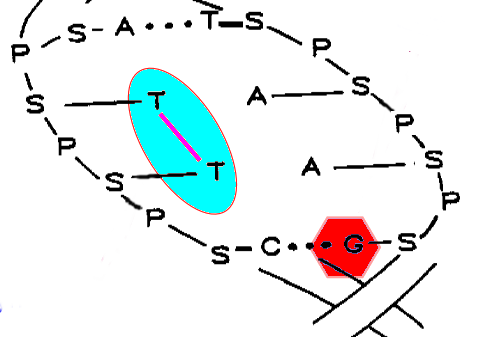
\includegraphics[width=0.5\linewidth]{./Figures/base-piri.png}
    \caption[Esquema Daño base y Dimeridos]{}
    \label{fig:esbdb}
\end{figure}

\subsection{Daño Celular}
\subsubsection{Reparación del ADN}
\subsubsection{Mecanismos de defensa}
\subsubsection{Respuesta adaptativa}
\subsubsection{Efectos de radiación ionizante en celulas no irradiadas}
\cite{willmari}
